\section{Valores de dispositivos o elementos}
\begin{figure}[H]
    \centering
    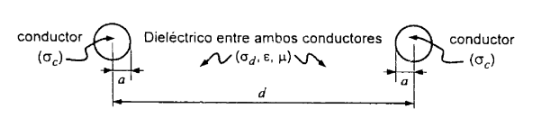
\includegraphics[width=5in]{lineasbifilares.png}
    \caption{Esquema de lineas bifilares}
    \label{fig:EsquemaBifilar}
\end{figure}

\begin{itemize}
    \item C=11 $\frac{pF}{m}$
    \item L=1 $\frac{\mu H}{m}$
    \item G=0 $\frac{S}{m}$
    \item R=0.8 $\Omega$
    \item a= 1mm
    \item d=12mm
    \item $\beta = 2.1386 \frac{rad}{m}$
    \item $\epsilon_r$ = 1,0412 (material del dieléctrico es aire)
    \item  $\sigma_c= 4,8x10^7$
\end{itemize}


\pagebreak